The training of recurrent neural networks is afflicted by the so called \textit{exploding} and \textit{vanishing} gradient problem.
Such problem is directly linked to the notion of memory. When we talk about memory what are we really talking about is the dependecy of neuron output at a given time $t$ from previous time steps,
that is how $\phi^t$ depends on $\phi^{k}$ with $t>k$. This dependecy is captured by the expression $\frac{\partial \vec{a}^t}{\partial \vec{a}^k}$.
Obiuvsly when such expression equals zero it means neuron output at time $t$ is not affected by output at time $k$.
The terms $\frac{\partial \vec{a}^t}{\partial \vec{a}^k}$ are usually referred as \textit{long term} contribution when $k<<t$ or \textit{short term} contributions
otherwise.
We talk of \textit{exploding} gradient problem when \textit{long term} components grow exponentially, on the contrary of \textit{short term} ones, causing
the overall norm of the gradient to explode.
We refer to \textit{vanishing} gradient problem when, vice versa, \textit{long terms} diminish exponentially.

\textit{Vanishing} gradient means long term components approach zero value, this in turn leads to the fact that the output of the net won't depend on inputs of distant temporal steps, i.e the output
sequence is determined only using recent temporal input: we say that the network doesn't have memory. Evidently this can have catastrofic effects on the classification error. Imagine we would like
to classiy an input sequence as positive wheter or not it contains a zero character. It would seem a rather easy task, a task other classification models wouldn't have difficulties with. If the neural network
we are trainign has \textit{vanishing} gradient issue, it means it perform classification only using the most recent temporal input. What if the zero character was at the beginning of the sequence? Of course
the predicition would be wrong.

\textit{Exploding} gradient seems to be a different kind of a problem, it does not affect the ability of the network to use information from distant temporal step, on the contrary we have very strong
information about where to go. One could argue that some components, namely, the long term ones, have gradient norm exponentially bigger than short term ones. I fail to see why this could be a problem:
of course output of the first timke stepes influences all successive steps, so changing the output of a long term neuron do imply big changes in the output of more distant in time neurons.
The only reason i see for considering this a problem is that big gradient norm, in general, is a problem if we are using algortithms like gradient descent with constant step.
If we are to compute a step in the gradient direction with a fixed step and gradient has too big norm we may make a too big step.

Let's now return to the nature of the problem and try to explaining the mechanics of it.

We have seen in the previous section that
\begin{equation}
\frac{\partial \vec{a}^t}{\partial \vec{a}^k} = \prod_{i=t-1}^{k}  diag(\sigma'(\vec{a}^i)) \cdot \mat{W}^{rec}
\label{memory_eq}
\end{equation}
Intuitively we can understand why such problems arises, more evidently in \textit{long term} components, just by looking at equation \ref{memory_eq};
We can notice each temporal contribution is the product of $l=t-k-1$ jacobian matrix, so in \textit{long term} components $l$ is large and depening on
eigenvalues of the matrixes in the product we can go exponentially fast towards 0 or infinty.


\paragraph{Explaining the problem using network's graph}
Let's now dig a bit deeper and rewrite equation \ref{memory_eq} with respect to a couple of neurons $i$ and $j$

\begin{equation} 
\frac{\partial \vec{a}_i^t}{\partial \vec{a}_j^k} = \sum_{q\in P(j)} \sum_{l \in P(q)} \hdots \sum_{h : i \in P(h)} w_{qj} \hdots w_{jh} \cdot \sigma'(a_j^k)\sigma'(a_q^{k+1}) \hdots \sigma'(a_i^{t-1})
\label{expanded_mem}
\end{equation}


Observing the previous equation we can argue that each derivatives it's the sum of $p^{t-k-1}$ terms; each term represents the path cost from neuron $i$ to neuron $j$ in the unfolded network, obviously
there are $p^{t-k-1}$ such paths. If we bind the cost $\sigma'(a_l^t)$ to neuron $l$ in the $t^{th}$ layer in the unfolded network we can read the path cost simply surfing the unfolded network multiply
the weight of each arc we walk through and the cost of each neuron we cross, as we can see from figure \ref{gradient_path_cost}.


\tikzstyle{rnn_style}=[->,shorten >=1pt,auto,node distance=1.5cm,
  thick,
  neuron/.style={circle,fill=white!50,draw,minimum size=0.7cm,inner sep=0pt,font=\sffamily\normalsize},
  missing/.style={circle,fill=white!50,draw=none,minimum size=0.7cm,font=\sffamily\Huge\bfseries},
  label/.style={node distance=1.2cm,rectangle,fill=white!50,draw=none,minimum size=0.7cm,font=\sffamily\normalsize},
  thick_edge/.style={line width=1.2pt},
  thin_edge/.style={dotted, line width=0.5pt},
  weight/.style = {above,sloped,pos=0.3},
  ]
\begin{figure}
 \centering
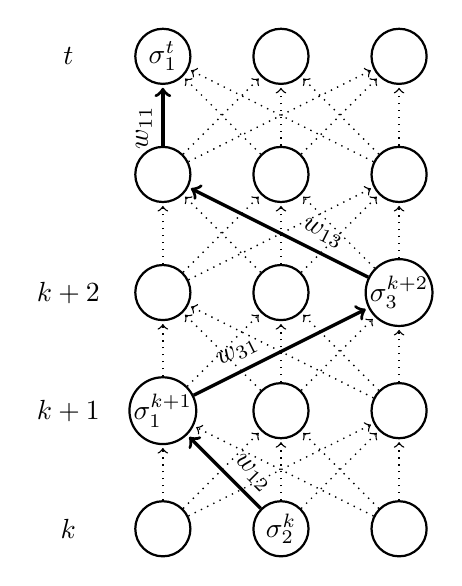
\begin{tikzpicture}[rnn_style]

  
  \node[neuron]    (x1)[]   {$\sigma_1^t$};
  \node[neuron]    (x2)[right of=x1]   {};
  \node[neuron]    (x3)[right of=x2]   {};
  \node[label]     (xl)[left of=x1] {$t$};
  
  \node[neuron]    (h1)[below of =x1]   {$\hdots$};
  \node[neuron]    (h2)[right of=h1]   {};
  \node[neuron]    (h3)[right of=h2]   {};
  \node[label]     (hl)[left of=h1] {$\hdots$};
  
  \node[neuron]    (y1)[below of=h1]   {};
  \node[neuron]    (y2)[right of=y1]   {};
  \node[neuron]    (y3)[right of=y2]   {$\sigma_3^{k+2}$};
  \node[label]     (yl)[left of=y1] {$k+2$};

  
  \node[neuron]    (z1)[below of=y1]   {$\sigma_1^{k+1}$};
  \node[neuron]    (z2)[right of=z1]   {};
  \node[neuron]    (z3)[right of=z2]   {};
  \node[label]     (zl)[left of=z1] {$k+1$};
  
  \node[neuron]    (w1)[below of=z1]   {};
  \node[neuron]    (w2)[right of=w1]   {$\sigma_2^k$};
  \node[neuron]    (w3)[right of=w2]   {};
  \node[label]     (wl)[left of=w1] {$k$};

  
%   \node[label]      (lu)[left of=u] {$u$};
%   \node[label]      (ll)[left of=z1] {$l$};


  \path[->] (h1) edge [thick_edge] node[weight]{$w_{11}$}  (x1)
	    (h1) edge [thin_edge]   (x2)
	    (h1) edge [thin_edge]   (x3)
	    (h2) edge [thin_edge]  (x1)
	    (h2) edge [thin_edge]   (x2)
	    (h2) edge [thin_edge]   (x3)
	    (h3) edge [thin_edge]  (x1)
	    (h3) edge [thin_edge]   (x2)
	    (h3) edge [thin_edge]   (x3);

  \path[->] (y1) edge [thin_edge]   (h1)
	    (y1) edge [thin_edge]   (h2)
	    (y1) edge [thin_edge]   (h3)
	    (y2) edge [thin_edge]   (h1)
	    (y2) edge [thin_edge]   (h2)
	    (y2) edge [thin_edge]   (h3)
	    (y3) edge [thick_edge] node[weight]{$w_{13}$}   (h1)
	    (y3) edge [thin_edge]   (h2)
	    (y3) edge [thin_edge]   (h3);
  
  
  \path[->] (z1) edge [thin_edge]   (y1)
	    (z1) edge [thin_edge]  (y2)
	    (z1) edge [thick_edge] node[weight]{$w_{31}$}   (y3)
	    (z2) edge [thin_edge]  (y1)
	    (z2) edge [thin_edge]  (y2)
	    (z2) edge [thin_edge]  (y3)
	    (z3) edge [thin_edge]   (y1)
	    (z3) edge [thin_edge]   (y2)
	    (z3) edge [thin_edge]   (y3);
	    
  \path[->] (w1) edge [thin_edge]   (z1)
	    (w1) edge [thin_edge]  (z2)
	    (w1) edge [thin_edge]   (z3)
	    (w2) edge [thick_edge] node[weight]{$w_{12}$}   (z1)
	    (w2) edge [thin_edge]   (z2)
	    (w2) edge [thin_edge]   (z3)
	    (w3) edge [thin_edge]   (z1)
	    (w3) edge [thin_edge]   (z2)
	    (w3) edge [thin_edge]   (z3);

	    


\end{tikzpicture}
\caption{The cost for a path from neuron $2$ at time $k$ to neuron $1$ at time $t$ is $w_{12}w_{31}w_{13}\hdots w_{11}\cdot \sigma_2^k \sigma_1^{k+1}\sigma_3^{k+2} \hdots \sigma_1^{t-1} $ }
\label{gradient_path_cost}
\end{figure}


We can further characterize each path cost noticing that we can separate two components, one that depends only on the weights $w_{qj} \hdots w_{jh}$ and the other that depends both on the weights and the inputs
$\sigma'(a_j^k)\sigma'(a_q^{k}) \hdots \sigma'(a_i^{t-1})$.


\paragraph{Hochreiter Analysis: Weak upper bound}
In this paragraph we report some useful consideration made by Hochreiter, please see \cite{Hochreiter95longshort-term} for more details.

Let's put:
$$\norm{\mat{A}}_{max}\triangleq \underset{i,j}{\text{max}}|a_{ij}| $$
$$\sigma'_{max} \triangleq \underset{i=k,...,t-1}{\text{max  }} \{\norm{diag(\sigma'(a^i))}_{max}\}$$
Since
\begin{align}
\norm{\mat{A}\cdot\mat{B}}_{max} &<= p \cdot \norm{\mat{A}}\cdot \norm{\mat{B}}_{max} & \forall \mat{A},\mat{B} \in \mathbb{R}_{p\times p} 
\end{align}
it holds:
\begin{align}
\norm{\frac{\partial \vec{a}^t}{\partial \vec{a}^k}}_{max} &= \norm{ \prod_{i=t-1}^{k}  diag(\sigma'(\vec{a}^i)) \cdot \mat{W}^{rec} }_{max}\\
&\leq \prod_{i=t-1}^{k} p \cdot \norm{diag(\sigma'(\vec{a}^i))}_{max} \cdot \norm{\mat{W}^{rec}}_{max}\\
&\leq \big(p \cdot \sigma'_{max} \cdot \norm{\mat{W}^{rec}}_{max}\big)^{t-k-1} \\
&= \tau^{t-k-1}
\end{align}
where $$\tau \triangleq p \cdot \sigma'_{max} \cdot \norm{\mat{W}^{rec}}_{max}$$

So we have exponential decay if $\tau<1$; We can match this condition if $\norm{\mat{W}^{rec}}_{max} \leq \frac{1}{p\cdot \sigma'_{max}}$
As pointed out by Hochreiter in his work we can match this condition, in the case of sigmoid activation function by choosing $\norm{\mat{W}^{rec}}_{max} < \frac{4}{p}$.

Let's note that we would actually reach this upper bound for some $i,j$ only if all the path cost have the same sign and the activations function take maximal
value.

\paragraph{The ReLU case}
ReLU case is a bit special, because of it's derivative.
ReLU's derivative is a step function, it can assume only two values: $1$ when the neuron is active, $0$ otherwise.
Returning to the path graph we introduced earlier we can say that a path is \textit{enabled} if each neuron in that path is active. In fact if we
encounter a path wich cross a non active neuron it's path cost will be 0; on the contrary for an \textit{enabled} path thw cost will be simply the product
of weight of the arcs we went through, as we can see in figure \ref{gradient_path_cost_relu}


\tikzstyle{rnn_style}=[->,shorten >=1pt,auto,node distance=1.5cm,
  thick,
  neuron/.style={circle,fill=white!50,draw,minimum size=0.7cm,inner sep=0pt,font=\sffamily\normalsize},
  missing/.style={circle,fill=white!50,draw=none,minimum size=0.7cm,font=\sffamily\Huge\bfseries},
  label/.style={node distance=1.2cm,rectangle,fill=white!50,draw=none,minimum size=0.7cm,font=\sffamily\normalsize},
  thick_edge/.style={line width=1.2pt},
  thin_edge/.style={dotted, line width=0.5pt},
  weight/.style = {above,sloped,pos=0.3},
  blacked/.style={fill=black},
  ]
\begin{figure}
 \centering
\begin{tikzpicture}[rnn_style]

  
  \node[neuron,blacked]    (x1)[]   {};
  \node[neuron]    (x2)[right of=x1]   {};
  \node[neuron]    (x3)[right of=x2]   {};
  \node[label]     (xl)[left of=x1] {$t$};
  
  \node[neuron,blacked]    (h1)[below of =x1]   {};
  \node[neuron]    (h2)[right of=h1]   {};
  \node[neuron]    (h3)[right of=h2]   {};
  \node[label]     (hl)[left of=h1] {$\hdots$};
  
  \node[neuron]    (y1)[below of=h1]   {};
  \node[neuron]    (y2)[right of=y1]   {};
  \node[neuron,blacked]    (y3)[right of=y2]   {};
  \node[label]     (yl)[left of=y1] {$k+2$};

  
  \node[neuron,blacked]    (z1)[below of=y1]   {};
  \node[neuron]    (z2)[right of=z1]   {};
  \node[neuron]    (z3)[right of=z2]   {};
  \node[label]     (zl)[left of=z1] {$k+1$};
  
  \node[neuron]    (w1)[below of=z1]   {};
  \node[neuron,blacked]    (w2)[right of=w1]   {};
  \node[neuron]    (w3)[right of=w2]   {};
  \node[label]     (wl)[left of=w1] {$k$};

  
%   \node[label]      (lu)[left of=u] {$u$};
%   \node[label]      (ll)[left of=z1] {$l$};


  \path[->] (h1) edge [thick_edge] node[weight]{$w_{11}$}  (x1)
	    (h1) edge [thin_edge]   (x2)
	    (h1) edge [thin_edge]   (x3)
	    (h2) edge [thin_edge]  (x1)
	    (h2) edge [thin_edge]   (x2)
	    (h2) edge [thin_edge]   (x3)
	    (h3) edge [thin_edge]  (x1)
	    (h3) edge [thin_edge]   (x2)
	    (h3) edge [thin_edge]   (x3);

  \path[->] (y1) edge [thin_edge]   (h1)
	    (y1) edge [thin_edge]   (h2)
	    (y1) edge [thin_edge]   (h3)
	    (y2) edge [thin_edge]   (h1)
	    (y2) edge [thin_edge]   (h2)
	    (y2) edge [thin_edge]   (h3)
	    (y3) edge [thick_edge] node[weight]{$w_{13}$}   (h1)
	    (y3) edge [thin_edge]   (h2)
	    (y3) edge [thin_edge]   (h3);
  
  
  \path[->] (z1) edge [thin_edge]   (y1)
	    (z1) edge [thin_edge]  (y2)
	    (z1) edge [thick_edge] node[weight]{$w_{31}$}   (y3)
	    (z2) edge [thin_edge]  (y1)
	    (z2) edge [thin_edge]  (y2)
	    (z2) edge [thin_edge]  (y3)
	    (z3) edge [thin_edge]   (y1)
	    (z3) edge [thin_edge]   (y2)
	    (z3) edge [thin_edge]   (y3);
	    
  \path[->] (w1) edge [thin_edge]   (z1)
	    (w1) edge [thin_edge]  (z2)
	    (w1) edge [thin_edge]   (z3)
	    (w2) edge [thick_edge] node[weight]{$w_{12}$}   (z1)
	    (w2) edge [thin_edge]   (z2)
	    (w2) edge [thin_edge]   (z3)
	    (w3) edge [thin_edge]   (z1)
	    (w3) edge [thin_edge]   (z2)
	    (w3) edge [thin_edge]   (z3);

	    


\end{tikzpicture}
\caption{The cost for an enabled path from neuron $2$ at time $k$ to neuron $1$ at time $t$ is $w_{12}w_{31}w_{13}\hdots w_{11}$ }
\label{gradient_path_cost_relu}
\end{figure}


So $\vert (\frac{\partial \vec{a}^t}{\partial \vec{a}^k})_{ij}\vert$ ranges from 0, when no path is enabled to, $\vert ((\mat{W}^{rec})^{t-k-1})_{ij} \vert$ when all
paths are enabled, which is consistent with what we found in Hochreiter analysis.

COMPORTAMENTO SBALIATO STRUTTURALE\\





